\documentclass[aspectratio=169,10pt]{beamer}

\usepackage{fontspec}
\usepackage{graphicx}
\usepackage{tikz}
\usepackage{booktabs}
\usepackage{array}
\usepackage{tabularx}
\usepackage{pgfplots}
\usepackage{fontawesome5}
\usepackage{ifthen}
\usepackage{hyperref}

\pgfplotsset{compat=1.18}
\usetikzlibrary{positioning}

\setsansfont{Source Sans 3}
\newfontfamily\titlefont{Montserrat}

\definecolor{TitleBlack}{HTML}{000000}
\definecolor{BodyGrey}{HTML}{65616A}
\definecolor{Accent}{HTML}{009689}
\definecolor{LightAccent}{HTML}{E8F7F5}
\definecolor{SoftGrey}{HTML}{F7F2FC}

\usetheme{default}
\usecolortheme{default}
\setbeamertemplate{navigation symbols}{}
\setbeamertemplate{footline}{%
  \begin{beamercolorbox}[wd=\paperwidth,ht=2.7ex,dp=1.1ex,leftskip=1.2em,rightskip=1.2em]{footline}%
    \color{BodyGrey}\scriptsize Chess Position Recognition\hfill\insertframenumber/\inserttotalframenumber
  \end{beamercolorbox}%
}
\setbeamertemplate{headline}{}
\setbeamertemplate{itemize item}{\color{Accent}\small\raisebox{0.1ex}{\faCircle}}
\setbeamertemplate{itemize subitem}{\color{Accent}\tiny\raisebox{0.1ex}{\faCircle}}

\setbeamercolor{background canvas}{bg=white}
\setbeamercolor{normal text}{fg=BodyGrey,bg=white}
\setbeamercolor{frametitle}{fg=TitleBlack,bg=white}
\setbeamercolor{title}{fg=TitleBlack,bg=white}
\setbeamercolor{subtitle}{fg=BodyGrey,bg=white}
\setbeamercolor{structure}{fg=Accent}
\setbeamerfont{title}{family=\titlefont,size=\Huge,series=\bfseries}
\setbeamerfont{subtitle}{size=\large}
\setbeamerfont{frametitle}{family=\titlefont,size=\Large,series=\bfseries}
\setbeamerfont{normal text}{size=\normalsize}

\hypersetup{colorlinks=true,linkcolor=Accent,urlcolor=Accent}

\newcommand{\SlideTitle}[1]{%
  \vspace{0.2em}%
  {\titlefont\color{TitleBlack}\Large\bfseries #1}\par\vspace{0.35em}%
  {\color{Accent}\rule{0.16\paperwidth}{1.4pt}}\vspace{0.7em}%
}

\newcommand{\MetricCard}[3]{%
  \begin{minipage}[t]{\linewidth}
    \begin{tikzpicture}
      \node[draw=Accent, fill=LightAccent, rounded corners=5pt, inner sep=7pt, text width=0.82\linewidth] {%
        {\titlefont\color{TitleBlack}\bfseries #1}\par\vspace{0.25em}%
        {\color{Accent}\Large\bfseries #2}\par\vspace{0.2em}%
        {\color{BodyGrey}\scriptsize #3}%
      };
    \end{tikzpicture}
  \end{minipage}%
}

\newcommand{\MaybeFigure}[3]{%
  \IfFileExists{#1}{%
    \includegraphics[width=#2]{#1}%
  }{%
    \begin{tikzpicture}
      \node[draw=Accent, fill=LightAccent, rounded corners=6pt, inner sep=10pt, text width=#2, minimum height=#3, align=center] {%
        {\titlefont\color{TitleBlack}\bfseries Pending generated figure}\par\vspace{0.4em}%
        {\color{BodyGrey}\small Run \texttt{just run}, then rerun \texttt{just presentation-build}.}\par\vspace{0.2em}%
        {\color{BodyGrey}\scriptsize #1}%
      };
    \end{tikzpicture}%
  }%
}

\title{Chess Position Recognition}
\subtitle{Square-level chessboard recognition with a scratch PyTorch CNN}
\author{Oğuzhan Özkaya}
\institute{ADA 447 Introduction to Deep Learning -- TED University}
\date{\today}

\begin{document}

\begin{frame}[plain]
  \vspace{1.5em}
  {\titlefont\color{TitleBlack}\Huge\bfseries Chess Position Recognition}\par
  \vspace{0.55em}
  {\color{Accent}\rule{0.38\paperwidth}{2pt}}\par
  \vspace{1em}
  {\color{BodyGrey}\Large Square-level board understanding from schematic chess images}\par
  \vfill
  \begin{tabular}{@{}ll@{}}
    \color{TitleBlack}\bfseries Dataset & \color{BodyGrey}Kaggle Chess Positions \\
    \color{TitleBlack}\bfseries Model & \color{BodyGrey}Scratch residual CNN in PyTorch \\
    \color{TitleBlack}\bfseries Primary metric & \color{BodyGrey}Square accuracy over 64 board cells \\
  \end{tabular}
  \vfill
  {\color{BodyGrey}\small Oğuzhan Özkaya \hfill ADA 447 Introduction to Deep Learning}
\end{frame}

\begin{frame}{Project Goal}
  \SlideTitle{Project Goal}
  \begin{columns}[T,onlytextwidth]
    \begin{column}{0.58\textwidth}
      \begin{itemize}
        \item Input: one aligned 400 by 400 RGB chessboard image.
        \item Output: one label for every board square.
        \item Label set: \texttt{empty}, white pieces, and black pieces.
        \item Success is measured primarily by square-level accuracy.
      \end{itemize}
    \end{column}
    \begin{column}{0.37\textwidth}
      \MetricCard{Prediction Target}{64}{squares per image}\par\vspace{0.25em}
      \MetricCard{Classes}{13}{empty + 12 pieces}\par\vspace{0.25em}
      \MetricCard{Main Metric}{Accuracy}{square-level correctness}
    \end{column}
  \end{columns}
\end{frame}

\begin{frame}{Dataset}
  \SlideTitle{Dataset}
  \begin{itemize}
    \item Source: \href{https://www.kaggle.com/datasets/koryakinp/chess-positions}{Chess Positions} dataset.
    \item 100,000 generated schematic board images.
    \item 80,000 training images and 20,000 test images.
    \item Each image contains 5--15 pieces, including both kings.
    \item Images span many board and piece style combinations.
    \item Filename stems encode labels as FEN ranks with dashes instead of slashes.
  \end{itemize}
\end{frame}

\begin{frame}{Data Contract}
  \SlideTitle{Data Contract}
  \begin{tabularx}{\textwidth}{@{}>{\bfseries\color{TitleBlack}}lX@{}}
    \toprule
    Field & Requirement \\
    \midrule
    Location & \texttt{data/train/} and \texttt{data/test/} \\
    Image & RGB board image, read from disk every run \\
    Label & Filename stem with 8 dash-separated FEN ranks \\
    Split & Random validation split from \texttt{data/train/}; final test uses \texttt{data/test/} \\
    Cache policy & No processed dataset cache is written \\
    \bottomrule
  \end{tabularx}
\end{frame}

\begin{frame}{Label Parsing}
  \SlideTitle{Label Parsing}
  \begin{columns}[T,onlytextwidth]
    \begin{column}{0.56\textwidth}
      \begin{itemize}
        \item A filename stem is split into 8 ranks.
        \item Digits expand to repeated \texttt{empty} squares.
        \item Piece letters map directly to class ids.
        \item The result is an \texttt{8 x 8} label grid.
      \end{itemize}
    \end{column}
    \begin{column}{0.4\textwidth}
      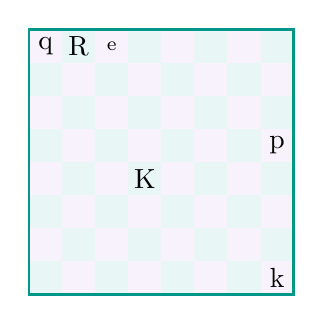
\begin{tikzpicture}[x=0.42cm,y=0.42cm]
        \foreach \x in {0,...,7} {
          \foreach \y in {0,...,7} {
            \pgfmathparse{mod(\x+\y,2)==0 ? "LightAccent" : "SoftGrey"}
            \edef\cellcolor{\pgfmathresult}
            \fill[\cellcolor] (\x,\y) rectangle +(1,1);
          }
        }
        \draw[Accent, line width=1pt] (0,0) rectangle (8,8);
        \node[color=TitleBlack] at (0.5,7.5) {q};
        \node[color=TitleBlack] at (1.5,7.5) {R};
        \node[color=TitleBlack] at (2.5,7.5) {\scriptsize e};
        \node[color=TitleBlack] at (7.5,4.5) {p};
        \node[color=TitleBlack] at (3.5,3.5) {K};
        \node[color=TitleBlack] at (7.5,0.5) {k};
      \end{tikzpicture}
      \par\vspace{0.7em}
      {\scriptsize\color{BodyGrey}\texttt{qR6-N7-...} becomes square labels.}
    \end{column}
  \end{columns}
\end{frame}

\begin{frame}{Pipeline}
  \SlideTitle{Pipeline}
  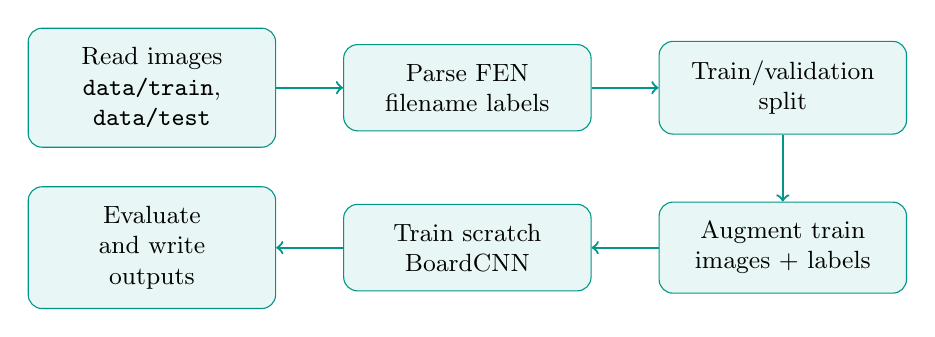
\begin{tikzpicture}[node distance=0.85cm, every node/.style={font=\small}]
    \tikzstyle{box}=[draw=Accent, fill=LightAccent, rounded corners=5pt, align=center, inner sep=7pt, text width=2.65cm]
    \node[box] (a) {Read images\\\texttt{data/train}, \texttt{data/test}};
    \node[box, right=of a] (b) {Parse FEN\\filename labels};
    \node[box, right=of b] (c) {Train/validation\\split};
    \node[box, below=of c] (d) {Augment train\\images + labels};
    \node[box, left=of d] (e) {Train scratch\\BoardCNN};
    \node[box, left=of e] (f) {Evaluate and write\\outputs};
    \draw[->, thick, Accent] (a) -- (b);
    \draw[->, thick, Accent] (b) -- (c);
    \draw[->, thick, Accent] (c) -- (d);
    \draw[->, thick, Accent] (d) -- (e);
    \draw[->, thick, Accent] (e) -- (f);
  \end{tikzpicture}
\end{frame}

\begin{frame}{Model Architecture}
  \SlideTitle{Model Architecture}
  \begin{columns}[T,onlytextwidth]
    \begin{column}{0.52\textwidth}
      \begin{itemize}
        \item Implemented directly in PyTorch as \texttt{BoardCNN}.
        \item Residual convolution blocks learn piece and board features.
        \item Spatial downsampling aligns features to an 8 by 8 grid.
        \item A 1 by 1 convolution emits class logits for each square.
      \end{itemize}
    \end{column}
    \begin{column}{0.44\textwidth}
      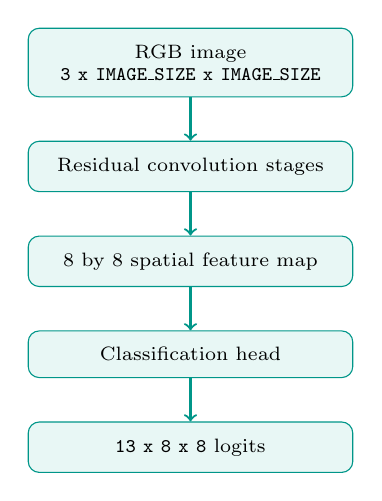
\begin{tikzpicture}[node distance=0.55cm, every node/.style={font=\scriptsize}]
        \tikzstyle{layer}=[draw=Accent, fill=LightAccent, rounded corners=4pt, align=center, inner sep=6pt, text width=3.7cm]
        \node[layer] (i) {RGB image\\\texttt{3 x IMAGE\_SIZE x IMAGE\_SIZE}};
        \node[layer, below=of i] (r) {Residual convolution stages};
        \node[layer, below=of r] (g) {8 by 8 spatial feature map};
        \node[layer, below=of g] (h) {Classification head};
        \node[layer, below=of h] (o) {\texttt{13 x 8 x 8} logits};
        \draw[->, thick, Accent] (i) -- (r);
        \draw[->, thick, Accent] (r) -- (g);
        \draw[->, thick, Accent] (g) -- (h);
        \draw[->, thick, Accent] (h) -- (o);
      \end{tikzpicture}
    \end{column}
  \end{columns}
\end{frame}

\begin{frame}{Training Setup}
  \SlideTitle{Training Setup}
  \begin{tabularx}{\textwidth}{@{}>{\bfseries\color{TitleBlack}}lX@{}}
    \toprule
    Component & Setting \\
    \midrule
    Optimizer & AdamW with weight decay \\
    Loss & Cross-entropy over square labels \\
    Empty handling & Lower empty-class weight to focus on occupied squares \\
    Regularization & Dropout, label smoothing, and label-preserving augmentation \\
    Hardware target & Local RTX 4080 with CUDA mixed precision \\
    Checkpoint rule & Best model selected by validation square accuracy \\
    \bottomrule
  \end{tabularx}
\end{frame}

\begin{frame}{Metrics}
  \SlideTitle{Metrics}
  \begin{itemize}
    \item \textbf{Square accuracy}: primary metric over every board square.
    \item \textbf{Occupied-square accuracy}: piece recognition without empty squares.
    \item \textbf{Empty-square accuracy}: empty-cell recognition quality.
    \item \textbf{Board accuracy}: strict metric requiring all 64 squares correct.
    \item \textbf{Per-class precision/recall/F1}: piece-specific behavior.
  \end{itemize}
\end{frame}

\begin{frame}{Generated Outputs}
  \SlideTitle{Generated Outputs}
  \begin{tabularx}{\textwidth}{@{}>{\bfseries\color{TitleBlack}}lX@{}}
    \toprule
    Path & Purpose \\
    \midrule
    \texttt{output/models/} & PyTorch checkpoints and final model \\
    \texttt{output/predictions/} & Square-level predictions in CSV and Parquet \\
    \texttt{output/reports/} & Metrics, class reports, and training history \\
    \texttt{output/figures/} & Training curves, confusion matrix, confidence plots \\
    \bottomrule
  \end{tabularx}
\end{frame}

\begin{frame}{Training Curves}
  \SlideTitle{Training Curves}
  \begin{columns}[T,onlytextwidth]
    \begin{column}{0.49\textwidth}
      \centering
      \MaybeFigure{output/figures/training_loss.png}{0.94\linewidth}{4.3cm}
    \end{column}
    \begin{column}{0.49\textwidth}
      \centering
      \MaybeFigure{output/figures/training_accuracy.png}{0.94\linewidth}{4.3cm}
    \end{column}
  \end{columns}
\end{frame}

\begin{frame}{Evaluation Figures}
  \SlideTitle{Evaluation Figures}
  \begin{columns}[T,onlytextwidth]
    \begin{column}{0.49\textwidth}
      \centering
      \MaybeFigure{output/figures/confusion_matrix.png}{0.9\linewidth}{4.5cm}
    \end{column}
    \begin{column}{0.49\textwidth}
      \centering
      \MaybeFigure{output/figures/prediction_confidence.png}{0.9\linewidth}{4.5cm}
    \end{column}
  \end{columns}
\end{frame}

\begin{frame}{Results Placeholder}
  \SlideTitle{Results Placeholder}
  \begin{tabularx}{\textwidth}{@{}lXXX@{}}
    \toprule
    \textbf{Split} & \textbf{Square Accuracy} & \textbf{Occupied Accuracy} & \textbf{Board Accuracy} \\
    \midrule
    Validation & From \texttt{metrics.csv} & After training & After training \\
    Test & From \texttt{metrics.csv} & After training & After training \\
    \bottomrule
  \end{tabularx}
  \vspace{1em}
  {\color{BodyGrey}\small Rebuild this deck after the long run with \texttt{just presentation-build}.}
\end{frame}

\begin{frame}{Risks and Mitigations}
  \SlideTitle{Risks and Mitigations}
  \begin{tabularx}{\textwidth}{@{}>{\bfseries\color{TitleBlack}}lX@{}}
    \toprule
    Risk & Mitigation \\
    \midrule
    Empty-square dominance & Down-weight empty class and track occupied-square accuracy \\
    Style variation & Train on all board and piece styles with color augmentation \\
    Overfitting & Validation split, dropout, label smoothing, early stopping \\
    Slow full training & Mixed precision and RTX 4080 local execution \\
    Report drift & Presentation references generated outputs directly \\
    \bottomrule
  \end{tabularx}
\end{frame}

\begin{frame}{Reproducibility}
  \SlideTitle{Reproducibility}
  \begin{itemize}
    \item Install environment: \texttt{just sync}
    \item Smoke test: \texttt{just smoke}
    \item Full training: \texttt{just run}
    \item Build docs: \texttt{just docs-build}
    \item Build presentation: \texttt{just presentation-build}
  \end{itemize}
  \vspace{1em}
  {\color{BodyGrey}\small The project reads raw images on each run and writes all report artifacts under \texttt{output/}.}
\end{frame}

\begin{frame}{Conclusion}
  \SlideTitle{Conclusion}
  \begin{itemize}
    \item The project has been migrated to chess board position recognition.
    \item The model predicts all 64 square labels with one scratch CNN.
    \item Accuracy is measured at square, occupied-square, empty-square, and full-board levels.
    \item The remaining project work is the long RTX 4080 training run and final result interpretation.
  \end{itemize}
\end{frame}

\begin{frame}[plain]
  \vfill
  {\titlefont\color{TitleBlack}\Huge\bfseries Questions}\par
  \vspace{0.7em}
  {\color{Accent}\rule{0.25\paperwidth}{2pt}}\par
  \vspace{1em}
  {\color{BodyGrey}\Large Chess Position Recognition}\par
  \vfill
\end{frame}

\end{document}
